\part[Implicits]{Internal Domain Specific Languages II - Implicits}

\section{DSLs}
\subsection{How to write a DSL?}
\begin{frame}{How to write a DSL?}
There are basically two techniques for writing internal DSLs:
\begin{enumerate}
  \item method chaining (fluent interfaces)
  \item object scoping
\end{enumerate}
\end{frame}

\begin{frame}[fragile]{Method chaining}
\onslide<1->\begin{lstlisting}
object DSL {
\end{lstlisting}
\onslide<2->\begin{lstlisting}
  class Flight {
    var source: String = ""
    var destination: String = ""
    def from(source: String): Flight = {
       this.source = source
       this
    }
    def to(destination: String): Flight = {
       this.destination = destination
       this
    }
    override def toString = 
       "Flight from " + source + " to " + destination
  }
\end{lstlisting}
\onslide<1->\begin{lstlisting}
}
scala> import DSL._
scala> val flight = (new Flight).from("Stuttgart").to("Berlin")
flight: DSL.Flight = Flight from Stuttgart to Berlin
\end{lstlisting}
\end{frame}

\begin{frame}[fragile]{Method chaining}
\begin{lstlisting}
object DSL {
  object Flight {
    def from(s: String) = new Flight(source = s)
  }
  class Flight(
    val source: String = "",
    val destination: String = "") {
    def from(source: String): Flight = 
      new Flight(source, destination)
      
    def to(d: String): Flight = 
      new Flight(source, destination)
      
    override def toString = 
       "Flight from " + source + " to " + destination
  }
}
\end{lstlisting}
\end{frame}

\begin{frame}[fragile]{Scala is well suited for DSLs}
\begin{lstlisting}
scala> import DSL._
import DSL._

scala> val flight  = Flight.from("Stuttgart").to("Berlin")
flight: DSL.Flight = Flight from Stuttgart to Berlin

scala> val flight  = Flight from ("Stuttgart") to ("Berlin")
flight: DSL.Flight = Flight from Stuttgart to Berlin

scala> val flight  = Flight from "Stuttgart" to "Berlin"
flight: DSL.Flight = Flight from Stuttgart to Berlin
\end{lstlisting}
\end{frame}

\begin{frame}[fragile]{Object scoping}
\onslide<1->\begin{lstlisting}
object DSL {
\end{lstlisting}
\onslide<2->\begin{lstlisting}
  def produce(e: Exception): Condition = new Condition(e)

  class Condition(e: Exception) {
    def when(condition: => Boolean): Unit = {
      if (condition)
        throw e
    }
  }
\end{lstlisting}
\onslide<1->\begin{lstlisting}
}
\end{lstlisting}
\onslide<1->\begin{lstlisting}
class Dog(name: String) {
  import DSL._
  produce(new WrongNameException) when name == null
}
class WrongNameException extends Exception
\end{lstlisting}
\end{frame}

\subsection{Example of DSLs in Scala}
\begin{frame}[fragile]{Baysick}
\begin{lstlisting}
object Lunar extends Baysick with App {

  10 PRINT "Welcome to Baysick Lunar Lander v0.9"
  20 LET ('dist := 100)
  30 LET ('v := 1)
  40 LET ('fuel := 1000)
  50 LET ('mass := 1000)

  60 PRINT "You are drifting towards the moon."

  70 PRINT "You must decide how much fuel to burn."
  80 PRINT "To accelerate enter a positive number"
  90 PRINT "To decelerate a negative"

  100 PRINT "Distance " % 'dist % "km, " % "Velocity " % 'v % "km/s, " % "Fuel " % % 'fuel
  110 INPUT 'burn
  120 IF ABS('burn) <= 'fuel THEN 150
  130 PRINT "You don't have that much fuel"
\end{lstlisting}
\end{frame}

\begin{frame}[fragile]{Baysick}
\begin{lstlisting}
  140 GOTO 100
  150 LET ('v := 'v + 'burn * 10 / ('fuel + 'mass))
  160 LET ('fuel := 'fuel - ABS('burn))
  170 LET ('dist := 'dist - 'v)
  180 IF 'dist > 0 THEN 100
  190 PRINT "You have hit the surface"
  200 IF 'v < 3 THEN 240
  210 PRINT "Hit surface too fast (" % 'v % ")km/s"
  220 PRINT "You Crashed!"

  230 GOTO 250
  240 PRINT "Well done"

  250 END

  RUN
  
}
\end{lstlisting}
\end{frame}

\begin{frame}[fragile]{ScalaTest}
\begin{lstlisting}
result should have length (3)
result should have size (10)
string should startWith ("Hello")
one should be < (7)
sevenDotOh should be (6.9 plusOrMinus 0.2)
map should contain key (1)
map should contain value ("Howdy")
mylist should not equal (yourList)
option should be (None)
evaluating { null.toString } should produce[NullPointerException]
\end{lstlisting}
\end{frame}

\begin{frame}[fragile]{Specs2}
\begin{lstlisting}
import org.specs2._

class HelloWorldSpec extends Specification { def is =

  "This is a specification to check the 'Hello world' string"	^
                                                               	     p^
  "The 'Hello world' string should"                            	     ^
    "contain 11 characters"                                    	     ! e1^
    "start with 'Hello'"                                       	     ! e2^
    "end with 'world'"                                         	     ! e3^
                                                               	     end

  def e1 = "Hello world" must have size(11)
  def e2 = "Hello world" must startWith("Hello")
  def e3 = "Hello world" must endWith("world")
}
\end{lstlisting}
\end{frame}

\section{Implicits}
\subsection{Pimp My Library}
\begin{frame}{Implicits}
\begin{block}{What problem do implicits try to solve?}
\highlight{Extending} \alert{closed} libraries
\end{block}
\begin{block}{How do they do it?}
When the code fails to compile, the compiler does not give up. It seeks help in
the so called \highlight{implicit scope}. If the compiler finds helper utilities
it \highlight{implicitly} inserts them into your code
\end{block}
\begin{block}{What is the implicit scope?}
The implicit scope is another \highlight{dimension} for values, variables,
methods and objects
\end{block}
\end{frame}

\begin{frame}[fragile]{Implicit Conversions}
\begin{block}{The library to extend}
Our guinea-pig library is the class \lstinline!String!
\end{block}
\begin{block}{The behaviour to add}
We want our strings to have the method \lstinline!extractUpperCase!
\end{block}
\begin{alertblock}{\lstinline!String! is final}
\lstinline!final class String! cannot be extended via inheritance or mixin
composition. Strings are closed for modification AND for extension.
\end{alertblock}
\end{frame}

\begin{frame}[fragile]{Implicit Conversions}
\begin{block}{Steps you would need to take in any OO language}
\begin{enumerate}
  \item Create a \lstinline!class StringWrapper(value: String)!
  \item add the \lstinline!def extractUpperCase! to \lstinline!StringWrapper!
  \item create the \lstinline!def convert(value: String): StringWrapper!
  \item call \lstinline!convert("GmbH").extractUpperCase!
\end{enumerate}
\end{block}
\begin{exampleblock}{Steps you would need to do in Scala to make it look good}
\begin{enumerate}
  \item insert the conversion method into the implicit scope
  \item call \lstinline!"GmbH".extractUpperCase!
\end{enumerate}
\end{exampleblock}
\end{frame}

\begin{frame}[fragile]{Implicit Conversions}
\begin{exampleblock}{Extending String}
\begin{lstlisting}
class StringWrapper(value: String) {
   def extractUpperCase = value filter { _.isUpper }
}
implicit def convert(value: String) = new StringWrapper(value)
\end{lstlisting}
\end{exampleblock}
\begin{exampleblock}{Using Extensions}
\begin{lstlisting}
scala> convert("HyperText Transfer Protocol").extractUpperCase
res0: String = HTTP

scala> "HyperText Transfer Protocol".extractUpperCase
res1: String = HTTP
\end{lstlisting}
\end{exampleblock}
\end{frame}

\begin{frame}[fragile]{Implicit Conversions}
\begin{exampleblock}{Extending String}
\begin{lstlisting}
class StringWrapper(value: String) {
   def extractUpperCase = value filter { _.isUpper }
}
implicit def convert(value: String) = new StringWrapper(value)
\end{lstlisting}
\end{exampleblock}
\begin{exampleblock}{Extending String (Scala 2.10 syntax)}
\begin{lstlisting}
implicit class StringWrapper(value: String) {
   def extractUpperCase = value filter { _.isUpper }
}
\end{lstlisting}
\end{exampleblock}
\end{frame}

\begin{frame}[fragile]{Implicit Conversions}
\begin{block}{\lstinline!Predef!}
The \lstinline!object Predef! from the Scala library is automatically imported
into every .scala file. \lstinline!Predef! inserts a lot of useful implicit
conversions into the implicit scope.
\end{block}
\begin{exampleblock}{\lstinline!Predef! - Primitive Widenings}
\begin{lstlisting}
implicit def int2long(x: Int): Long = x.toLong
implicit def int2float(x: Int): Float = x.toFloat
implicit def int2double(x: Int): Double = x.toDouble
\end{lstlisting}
\end{exampleblock}
\end{frame}

\begin{frame}{Implicit Conversions - Views in Scala's Hierarchy}
\begin{center}
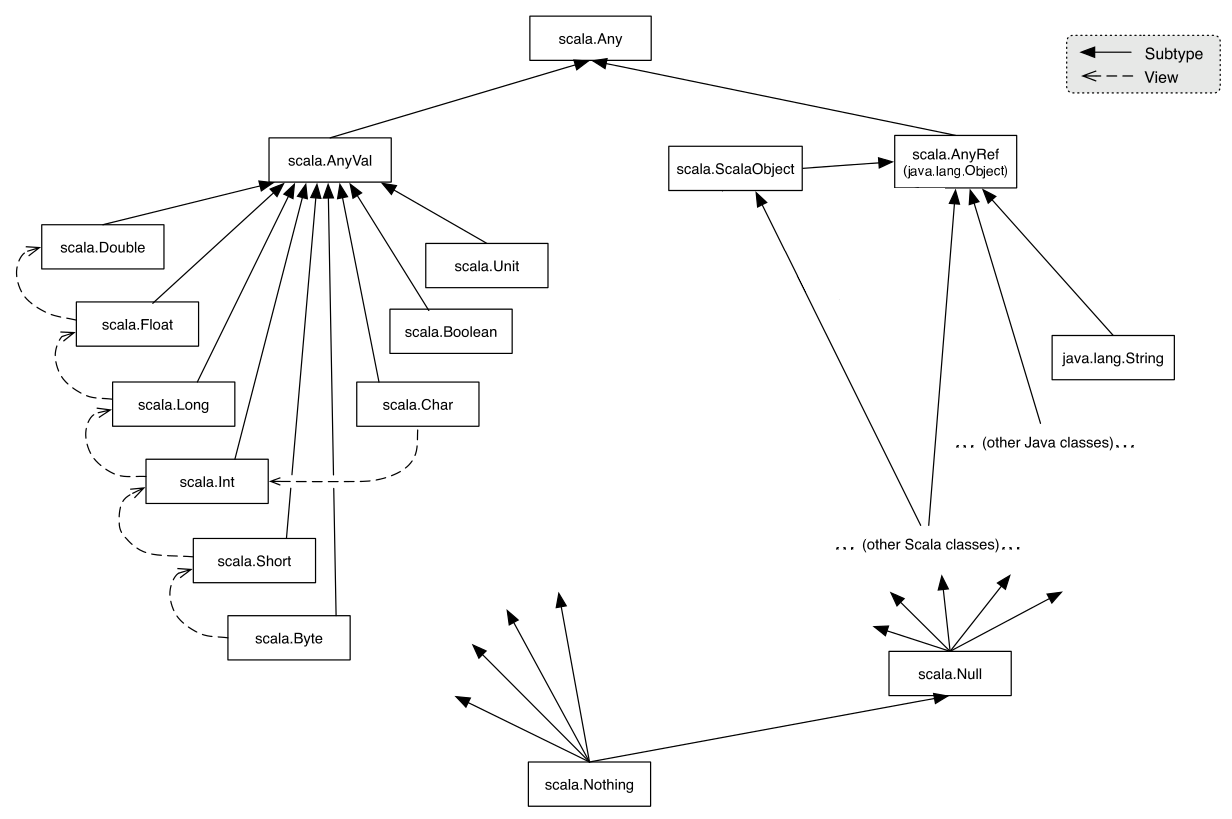
\includegraphics[width=\textwidth]{resources/Hierarchy.png}
\end{center}
\end{frame}

\begin{frame}[fragile]{Implicit Conversions - Further examples}
\begin{exampleblock}{\lstinline!Predef! - \lstinline!StringOps!}
\begin{lstlisting}
implicit def augmentString(x: String): StringOps = new StringOps(x)
implicit def unaugmentString(x: StringOps): String = x.repr
\end{lstlisting}
\end{exampleblock}

\begin{exampleblock}{\lstinline!Predef! - \lstinline!StringOps!}
\begin{lstlisting}
scala> val names = Seq("George", "Bob", "Frank")
names: Seq[String] = List(George, Bob, Frank)

scala> names forall { _.exists { _.isUpper } }
res0: Boolean = true
\end{lstlisting}
\end{exampleblock}
\end{frame}

\begin{frame}[fragile]{Implicit Conversions - Further examples}
\begin{exampleblock}{\lstinline!Predef! - \lstinline!RichInt!}
\begin{lstlisting}
implicit def intWrapper(x: Int): RichInt 
\end{lstlisting}
\end{exampleblock}

\begin{exampleblock}{\lstinline!Predef! - \lstinline!RichInt!}
\begin{lstlisting}
scala> 1 to 3
res0: immutable.Range.Inclusive = Range(1, 2, 3)

scala> 3 min 5
res1: Int = 3

scala> val bestNumberInBinary = 73.toBinaryString
bestNumberInBinary: String = 1001001

scala> bestNumberInBinary.size
res2: Int = 7

scala> bestNumberInBinary filter { _ == '1' } size
res3: Int = 3
\end{lstlisting}
\end{exampleblock}
\end{frame}

\begin{frame}[fragile]{Implicit Conversions - Further examples}
\begin{alertblock}{Everything is a Unit}
\begin{lstlisting}
scala> def x: Unit = 10
x: Unit
\end{lstlisting}
\end{alertblock}
\begin{alertblock}{Do not forget the equals sign}
\begin{lstlisting}
scala> def x { 10 }
x: Unit
\end{lstlisting}
\end{alertblock}
\end{frame}

\subsection{Rules for Implicits}
\begin{frame}[fragile]{Rules for Implicits I - Marking Rule}
\begin{block}{Marking Rule}
Only definitions marked implicit are available
\end{block}
\begin{exampleblock}{Considered during implicit look up}
\lstinline!implicit def convert(x: Int): String = x.toString!
\end{exampleblock}
\begin{alertblock}{Not considered during implicit look up}
\lstinline!def convert(x: Int): String = x.toString!
\end{alertblock}

\end{frame}

\begin{frame}[fragile]{Rules for Implicits II - Scope Rule}
\begin{block}{Scope Rule}
An inserted implicit conversion must be \highlight{in scope} as a
\highlight{single identifier}, or be associated with the source or target type
of the conversion
\end{block}
\begin{exampleblock}{Single identifier}
\lstinline!convert(x) + y!
\end{exampleblock}
\begin{alertblock}{Not a single identifier}
\lstinline!someObject.convert(x) + y!
\end{alertblock}
\begin{block}{Association with the source or target type}
Implicit conversions within \highlight{companion objects} are automatically
imported into the implicit scope
\end{block}
\end{frame}

\begin{frame}[fragile]{Rules for Implicits III - Not-Ambiguity Rule}
\begin{block}{Not-Ambiguity Rule}
An implicit conversion is only inserted if there is no other possible conversion
to insert
\end{block}
\begin{lstlisting}
implicit def convert1(x: Int) = new { def m = 1 }
implicit def convert2(x: Int) = new { def m = 2 }
\end{lstlisting}
\begin{alertblock}{Ambiguity violation}
\begin{lstlisting}
scala> 4711.m
<console>:10: error: type mismatch;
...
Note that implicit conversions are not applicable because
they are ambiguous:
 both method convert1 in object $iw of type
  (x: Int)java.lang.Object{def m: Int}
  and method convert2 in object $iw of type
  (x: Int)java.lang.Object{def m: Int}
 are possible conversion functions from Int(4711) to ?{val m: ?}
\end{lstlisting}
\end{alertblock}
\end{frame}

\begin{frame}[fragile]{Rules for Implicits IV - One-at-a-time Rule}
\begin{block}{One-at-a-time Rule}
Only one implicit is tried
\end{block}
\begin{alertblock}{One-at-a-time Rule violation}
\begin{lstlisting}
x + y // never gets rewritten as
convert1(convert2(x)) + y
\end{lstlisting}
\end{alertblock}
\end{frame}

\begin{frame}[fragile]{Rules for Implicits V - Explicit-First Rule}
\begin{block}{One-at-a-time Rule}
Whenever code type checks as it is written, no implicits are attempted
\end{block}
\begin{block}{Where implicits are tried}
\begin{enumerate}
  \item conversion to an expected type (call \lstinline!m(a: A)! with \lstinline!b: B!)
  \item conversion of the receiver of a selection (call \lstinline!a.m! when \lstinline!a! has no \lstinline!m!)
  \item implicit parameter lists (call \lstinline!m(a: A)(b: B)! like \lstinline!m(a: A)!)
\end{enumerate}
\end{block}
\end{frame}

\section{Typeclasses}
\begin{frame}[fragile]{Typeclasses}
\begin{block}{What are typeclasses?}
Haskell: Type class (language feature)\\
Scala: Typeclass (pattern)
\end{block}
\begin{block}{What is the typeclasses pattern?}
Adapter pattern with implicit sugar
\end{block}
\begin{block}{What are typeclasses trying to achieve?}
Typeclasses are a pattern for \highlight{decoupling} ad hoc polymorphism
\end{block}

\end{frame}

\begin{frame}[fragile]{Typeclasses by example}
\begin{block}{What is an algebraic data type?}
Algebraic data type is a type defined by providing \highlight{several
alternatives}, each of which comes with its \highlight{own constructor}. It
usually comes with a way to \highlight{decompose the type through pattern
matching}. Algebraic data types can be emulated in Scala with case classes.
\end{block}
\begin{exampleblock}{The \lstinline!Shape! ADT}
\begin{lstlisting}
sealed trait Shape
case object Point								extends Shape
case class Line(length: Int)					extends Shape
case class Square(side: Int)					extends Shape
case class Circle(radius: Int)					extends Shape
case class Rectangle(height: Int, width: Int)	extends Shape
\end{lstlisting}
\end{exampleblock}
\end{frame}

\begin{frame}[fragile]{Typeclasses by example}
\begin{alertblock}{AreaCalculator does not know anything about the ADT}
\begin{lstlisting}
object AreaCalculator {
  // How to calculate the area without knowing
  // what the type of shape is?
  // T is not even required to be a shape at all
  def calculateArea[T](shape: T): Double = ???
}
\end{lstlisting}
\end{alertblock}
\end{frame}

\begin{frame}[fragile]{Typeclasses by example}
\begin{block}{AreaConverter}
\begin{lstlisting}
trait AreaConverter[T] {
  def calculateArea(shape: T): Double
}
\end{lstlisting}
\end{block}
\begin{block}{AreaCalculator STILL does not know anything about the ADT}
\begin{lstlisting}
object AreaCalculator {
  def calculateArea[T](shape: T)(converter: AreaConverter[T]) =
    converter.calculateArea(shape)
}
\end{lstlisting}
\end{block}
\end{frame}

\begin{frame}[fragile]{Typeclasses by example}
\begin{block}{AreaConverter is a typeCLASS}
\begin{lstlisting}
trait AreaConverter[T] {
  def calculateArea(shape: T): Double
}
\end{lstlisting}
\end{block}
\begin{block}{These are the INSTANCES of AreaConverter typeclass}
\begin{lstlisting}
object SquareAreaConverter extends AreaConverter[Square] {
  def calculateArea(s: Square) = s.side * s.side
}

object CircleAreaConverter extends AreaConverter[Circle] {
  def calculateArea(c: Circle) = math.Pi * c.radius * c.radius
}

object RectangleAreaConverter extends AreaConverter[Rectangle] {
  def calculateArea(r: Rectangle) = r.height * r.width
}
\end{lstlisting}
\end{block}
\end{frame}

\begin{frame}[fragile]{Typeclasses by example}
\begin{block}{The adapter pattern is way too explicit}
\begin{lstlisting}
scala> import AreaCalculator._
import AreaCalculator._

scala> calculateArea(Circle(10))(CircleAreaConverter)
res0: Double = 314.1592653589793

scala> calculateArea(Square(5))(SquareAreaConverter)
res1: Double = 25.0

scala> calculateArea(Rectangle(5, 10))(RectangleAreaConverter)
res2: Double = 50.0
\end{lstlisting}
\end{block}
\end{frame}

\begin{frame}[fragile]{Typeclasses by example}
\begin{exampleblock}{AreaCalculator with implicit parameter}
\begin{lstlisting}
object AreaCalculator {
  def calculateArea[T](shape: T)
    (implicit converter: AreaConverter[T]) =
      converter.calculateArea(shape)
}
\end{lstlisting}
\end{exampleblock}
\begin{exampleblock}{AreaConverter instances are implicit now}
\begin{lstlisting}
implicit object SquareAreaConverter extends AreaConverter[Square] {
  def calculateArea(s: Square) = s.side * s.side
}
implicit object CircleAreaConverter extends AreaConverter[Circle] {
  def calculateArea(c: Circle) = math.Pi * c.radius * c.radius
}
implicit object RectangleAreaConverter extends AreaConverter[Rectangle] {
  def calculateArea(r: Rectangle) = r.height * r.width
}
\end{lstlisting}
\end{exampleblock}
\end{frame}

\begin{frame}[fragile]{Typeclasses by example}
\begin{exampleblock}{The typeclass pattern is the implicit adapter pattern}
\begin{lstlisting}
scala> import AreaCalculator._
import AreaCalculator._

scala> calculateArea(Circle(10))
res0: Double = 314.1592653589793

scala> calculateArea(Square(5))
res1: Double = 25.0

scala> calculateArea(Rectangle(5, 10))
res2: Double = 50.0
\end{lstlisting}
\end{exampleblock}
\end{frame}

\begin{frame}[fragile]{Typeclasses by example}
\begin{exampleblock}{AreaConverter}
\begin{lstlisting}
trait AreaConverter[T] {
  def calculateArea(shape: T): Double
}
\end{lstlisting}
\end{exampleblock}
\begin{exampleblock}{AreaCalculator}
\begin{lstlisting}
object AreaCalculator {
  def calculateArea[T](shape: T)
    (implicit conv: AreaConverter[T]) = conv.calculateArea(shape)
}
\end{lstlisting}
\end{exampleblock}
\begin{exampleblock}{AreaCalculator with some sugar}
\begin{lstlisting}
object AreaCalculator {
  def calculateArea[T : AreaConverter](shape: T) =
    implicitly[AreaConverter[T]].calculateArea(shape)
}
\end{lstlisting}
\end{exampleblock}
\end{frame}

\begin{frame}[fragile]{Typeclasses by example}
\begin{exampleblock}{AreaConverter}
\begin{lstlisting}
trait ShapeView[T] {
  def calculateArea(shape: T): Double
}
\end{lstlisting}
\end{exampleblock}
\begin{exampleblock}{AreaCalculator}
\begin{lstlisting}
object AreaCalculator {
  def calculateArea[T](shape: T)
    (implicit view: ShapeView[T]) = view.calculateArea(shape)
}
\end{lstlisting}
\end{exampleblock}
\begin{exampleblock}{AreaCalculator with some sugar}
\begin{lstlisting}
object AreaCalculator {
  def calculateArea[T : ShapeView](shape: T) =
    implicitly[ShapeView[T]].calculateArea(shape)
}
\end{lstlisting}
\end{exampleblock}
\end{frame}

\begin{frame}{TODO}
\begin{itemize}
  \item scopes
  \item refactoring
  \item views vllt
\end{itemize}
\end{frame}

\section{Summary}
\begin{frame}{Summary}
\begin{itemize}
  \item
\end{itemize}
\end{frame}